\documentclass[tikz]{standalone}
\usetikzlibrary{positioning}
\usepackage{amsmath}
\usepackage{mathrsfs}

\newcommand{\cat}[1]{\mathscr{#1}}
\newcommand{\obj}[1]{|#1|}
\newcommand{\mrp}[3]{#1(#2,#3)}
\newcommand{\id}[1]{\mathrm{id}_{#1}}
\DeclareMathOperator{\dom}{dom}
\DeclareMathOperator{\cod}{cod}
\DeclareMathOperator{\colim}{Colim}
\DeclareMathOperator{\lan}{Lan}
\DeclareMathOperator{\ran}{Ran}


\begin{document}
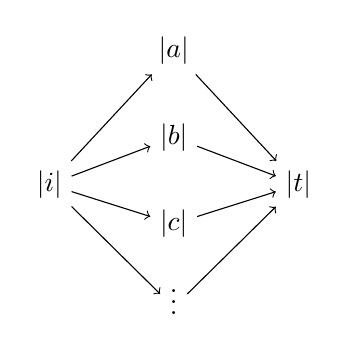
\begin{tikzpicture}
	\node (A) {$\obj{a}$};
	\node [below=0.5cm of A] (B) {$\obj{b}$};
	\node [below=0.5cm of B] (C) {$\obj{c}$};
	\node [below=0.2cm of C] (D) {$\vdots$};
	\node [below left =0.0cm and 1.0cm of B] (I) {$\obj{i}$};
	\node [below right=0.0cm and 1.0cm of B] (T) {$\obj{t}$};
	\draw [->] (I) to (A);
	\draw [->] (I) to (B);
	\draw [->] (I) to (C);
	\draw [->] (I) to (D.west);
	\draw [->] (A) to (T);
	\draw [->] (B) to (T);
	\draw [->] (C) to (T);
	\draw [->] (D.east) to (T);
\end{tikzpicture}
\end{document}
